\documentclass[border=10pt]{standalone}
\usepackage[european]{circuitikz}
\begin{document}
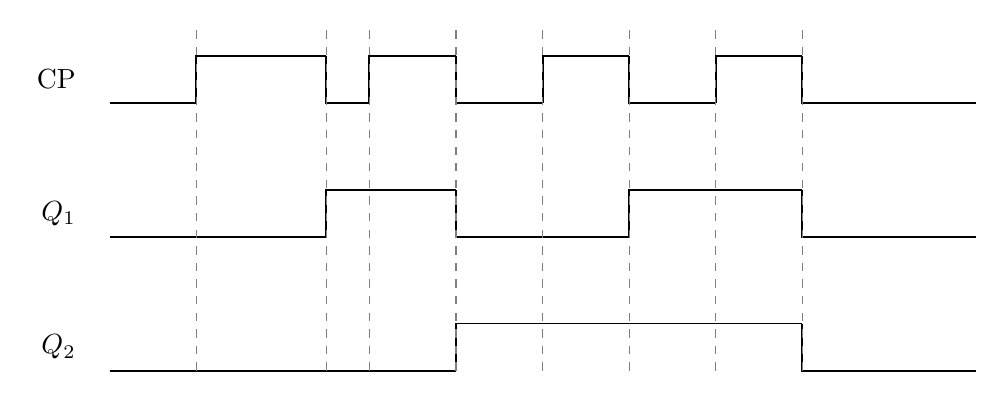
\begin{tikzpicture}[line width=0.7pt, font=\normalsize]

% 习题 8.8 答案波形：CP / Q₁ / Q₂ 三行，20 格等分 0–100%
%   CP 沿用 fig-8-02：四脉冲 10–25/30–40/50–60/70–80%
%   Q₁：初 0；25/40/60/80% 四个下降沿翻转 ⇒ 0→1→0→1→0
%   Q₂：只在 Q₁ 的下降沿 40/80% 翻转 ⇒ 0→1（40%）→0（80%）
%   竖虚线在 10/25/30/40/50/60/70/80% 八处（对齐四沿）
% 坐标：seg=0.55cm/格，总宽 11.0cm；行高 0.6，行距 1.7

\def\seg{0.55}
\def\hi{0.6}
\def\total{11.0}

% 电平段绘制宏：#1 y偏移  #2 标签  #3 电平串(段边界格号,竖线位置) —— 直接列点位
\newcommand{\wave}[3]{%
  \begin{scope}[yshift=#1cm]
    \node[anchor=east] at (-0.3,\hi/2) {#2};
    #3
  \end{scope}}

% CP：0-10 低 |10-25 高 |25-30 低 |30-40 高 |40-50 低 |50-60 高 |60-70 低 |70-80 高 |80-100 低
\wave{0}{CP}{%
  \draw (0,0) -- (2*\seg,0);
  \draw (2*\seg,0) -- (2*\seg,\hi) -- (5*\seg,\hi);
  \draw (5*\seg,\hi) -- (5*\seg,0) -- (6*\seg,0);
  \draw (6*\seg,0) -- (6*\seg,\hi) -- (8*\seg,\hi);
  \draw (8*\seg,\hi) -- (8*\seg,0) -- (10*\seg,0);
  \draw (10*\seg,0) -- (10*\seg,\hi) -- (12*\seg,\hi);
  \draw (12*\seg,\hi) -- (12*\seg,0) -- (14*\seg,0);
  \draw (14*\seg,0) -- (14*\seg,\hi) -- (16*\seg,\hi);
  \draw (16*\seg,\hi) -- (16*\seg,0) -- (\total,0);}

% Q₁：0-25 低 |25-40 高 |40-60 低 |60-80 高 |80-100 低
\wave{-1.7}{$Q_1$}{%
  \draw (0,0) -- (5*\seg,0);
  \draw (5*\seg,0) -- (5*\seg,\hi) -- (8*\seg,\hi);
  \draw (8*\seg,\hi) -- (8*\seg,0) -- (12*\seg,0);
  \draw (12*\seg,0) -- (12*\seg,\hi) -- (16*\seg,\hi);
  \draw (16*\seg,\hi) -- (16*\seg,0) -- (\total,0);}

% Q₂：0-40 低 |40-80 高 |80-100 低
\wave{-3.4}{$Q_2$}{%
  \draw (0,0) -- (8*\seg,0);
  \draw (8*\seg,0) -- (8*\seg,\hi) -- (16*\seg,\hi);
  \draw (16*\seg,\hi) -- (16*\seg,0) -- (\total,0);}

% 八条竖虚线（贯穿三行，不压字：画在波形之后、行间空白）
\foreach \g in {2,5,6,8,10,12,14,16} {
  \draw[dashed, gray, line width=0.4pt] (\g*\seg,-3.4) -- (\g*\seg,0.95);
}

\end{tikzpicture}
\end{document}
